\subsection{Punto de equilibrio}

Determinar el punto de equilibrio es esencial, ya que permite a la empresa conocer cuántas veces debe cubrir sus costos fijos operativos. Este análisis es clave para identificar el momento en que las ventas comenzarán a generar utilidades. En la tabla \ref{costosFijosVariables} se presentan las estimaciones de los costos fijos y variables asociados a las ventas del primer año.

\vspace{2mm}
\begin{minipage}{0.9\textwidth}
\centering
\captionof{table}[{Costos fijos y variables}]{ Costos fijos y variables. }
\label{costosFijosVariables}
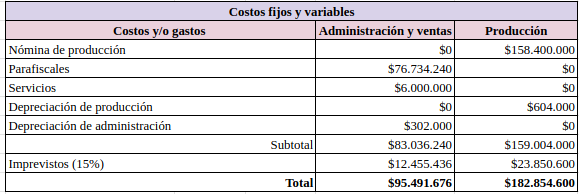
\includegraphics[width=0.9\textwidth]{Content/Images/AF/PuntoDeEquilibrio_CostosFijosYVar.png}
\footnote{Nota. \textup{Fuente : Autores}}
\end{minipage}

El costo fijo por unidad se obtiene al sumar los costos administrativos y de ventas, lo que permite calcular el costo total por unidad. Se estima un margen de valor agregado del 19\% (\$32.169), estableciendo un precio de venta de \$201.479. Para recuperar la inversión inicial, es necesario alcanzar 1.644 ventas anuales; a partir de ese punto, las ventas comenzarán a generar utilidades.

\vspace{2mm}
\begin{minipage}{0.9\textwidth}
\centering
\captionof{table}[{Estimaciones punto de equilibrio}]{ Estimaciones punto de equilibrio. }
\label{calculosPuntoEquilirbio}
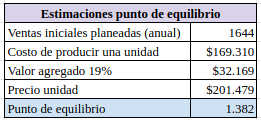
\includegraphics[width=0.9\textwidth]{Content/Images/AF/PuntoDeEquilibrio_Estimacion.png}
\footnote{Nota. \textup{Fuente : Autores}}
\end{minipage}

La gráfica muestra el punto de equilibrio mediante las líneas de costos totales y ventas. El eje X representa las unidades vendidas y el eje Y el monto en dinero; con 958 ventas, ambas líneas se igualan, marcando el punto de equilibrio.

\vspace{2mm}
\begin{minipage}{0.9\textwidth}
\centering
\captionof{table}[{Gráfica punto de equilibrio. }]{Gráfica punto de equilibrio. }
\label{graficaEquilibrio}
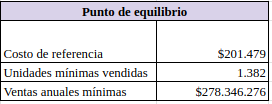
\includegraphics[width=0.9\textwidth]{Content/Images/AF/PuntoDeEquilibrio_PuntoDeEqui.png}
\footnote{Nota. \textup{Fuente : Autores}}
\end{minipage}

A partir de los resultados de la tabla \ref{puntoEquilibrio}, se sintetiza la información necesaria para calcular el punto de equilibrio.

\vspace{2mm}
\begin{minipage}{0.9\textwidth}
\centering
\captionof{table}[{Punto de equilibrio}]{ Punto de equilibrio. }
\label{puntoEquilibrio}
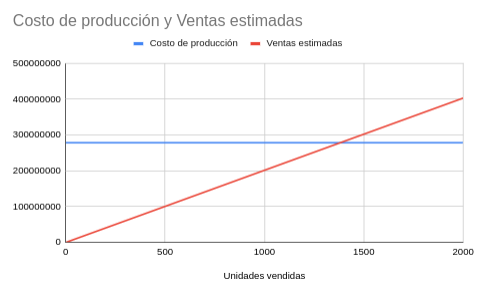
\includegraphics[width=0.9\textwidth]{Content/Images/AF/PuntoDeEquilibrio_CostosYVentas.png}
\footnote{Nota. \textup{Fuente : Autores}}
\end{minipage}